% ============================================================================
% Lecture 13 (B12): OLG Models with DEQNs
% Deep Learning for Solving and Estimating Dynamic Models in Economics and Finance
% Course author: Simon Scheidegger
% ============================================================================

\documentclass[aspectratio=169,11pt]{beamer}

% ---------- Theme and colors ----------
\usecolortheme{dove}
\setbeamertemplate{navigation symbols}{}
\setbeamertemplate{footline}{%
  \hfill\usebeamerfont{page number in head/foot}%
  \usebeamercolor[fg]{normal text}%
  \insertframenumber\,/\,\inserttotalframenumber\kern1em\vskip4pt}
\setbeamerfont{frametitle}{size=\huge}

% ---------- Packages ----------
\usepackage[utf8]{inputenc}
\usepackage[T1]{fontenc}
\usepackage{lmodern}
\usepackage{amsmath,amssymb,amsfonts}
\usepackage{bm}
\usepackage{graphicx}
\usepackage{tikz}
\usetikzlibrary{shapes,arrows.meta,positioning,calc,fit,backgrounds,patterns,decorations.pathreplacing}
\usepackage{pgfplots}
\pgfplotsset{compat=1.18}
\usepackage{booktabs}
\usepackage{hyperref}
\usepackage{xcolor}

% ---------- Custom colors ----------
\definecolor{uzhblue}{rgb}{0,0,0.5}
\definecolor{uzhgreylight}{RGB}{236,238,241}
\definecolor{uzhgreydark}{RGB}{81,86,94}
\definecolor{harvardcrimson}{RGB}{153,0,0}
\definecolor{unil@blue}{RGB}{0,140,204}
\definecolor{unil@black}{RGB}{35,31,32}
\definecolor{darkgreen}{RGB}{0,100,0}
\definecolor{darkred}{RGB}{139,0,0}
\definecolor{softblue}{RGB}{70,130,180}
\definecolor{softorange}{RGB}{230,159,0}
\definecolor{softgreen}{RGB}{0,158,115}

% ---------- Set beamer colors ----------
\setbeamercolor{frametitle}{bg=uzhgreylight, fg=uzhblue}
\setbeamercolor{title}{fg=uzhblue}
\setbeamercolor{structure}{fg=uzhblue}
\setbeamercolor{block title}{bg=unil@blue, fg=white}
\setbeamercolor{block body}{bg=uzhgreylight}
\setbeamercolor{block title alerted}{bg=darkred,fg=white}
\setbeamercolor{block body alerted}{bg=red!5}
\setbeamercolor{block title example}{bg=darkgreen,fg=white}
\setbeamercolor{block body example}{bg=green!5}
\setbeamercolor{item}{fg=unil@black}
\setbeamercolor{normal text}{fg=unil@black}

% ---------- Emphasis and hyperlinks ----------
\newcommand{\emphc}[1]{\textcolor{harvardcrimson}{#1}}
\hypersetup{colorlinks,linkcolor=harvardcrimson,urlcolor=harvardcrimson}

% ---------- Math shortcuts ----------
\newcommand{\R}{\mathbb{R}}
\newcommand{\E}[1]{\mathbb{E}\!\left[#1\right]}
\newcommand{\N}{\mathcal{N}}
\newcommand{\Loss}{\mathcal{L}}
\newcommand{\st}{\text{s.t.}\ }
\newcommand{\ubr}[2]{\underbrace{#1}_{\text{\scriptsize #2}}}

% ---------- Title ----------
\title[Lecture 08 (B07)]{Lecture 08 (B07): OLG models with DEQNs}
\subtitle{Overlapping generations, borrowing constraints, Fischer--Burmeister complementarity}
\author{Simon Scheidegger}
\institute{HEC, University of Lausanne}
\date{}
\begin{document}

% Custom command used in some "Finger Exercise" frame titles.
\providecommand{\exercisepause}{%
  \tikz[baseline=(X.base)]{\node[fill=darkgreen!80!black, text=white,
  rounded corners=2pt, inner sep=3pt, font=\scriptsize\bfseries](X){PAUSE};}}

{\setbeamercolor{background canvas}{bg=uzhgreylight}
\begin{frame}
\titlepage
\end{frame}
}

% --- About-this-lecture orientation ---

\begin{frame}{Roadmap}
\footnotesize
\begin{block}{Part I --- What is an OLG model?}
\vspace{-3pt}\begin{itemize}\itemsep0pt
    \item Why overlapping generations; cohort structure; the DEQN recipe in one line.
\end{itemize}
\end{block}
\vspace{-2pt}
\begin{block}{Part II --- The analytic 6-agent model (Krueger \& K\"ubler, 2004)}
\vspace{-3pt}\begin{itemize}\itemsep0pt
    \item Model $\to$ equilibrium $\to$ cost $\to$ FREE $\to$ architecture $\to$ training $\to$ validation against the closed form.
    \item Notebook: \texttt{07\_OLG\_Analytic\_DEQN.ipynb}.
\end{itemize}
\end{block}
\vspace{-2pt}
\begin{block}{Part III --- The leading example of AGS (2022): the 56-cohort benchmark}
\vspace{-3pt}\begin{itemize}\itemsep0pt
    \item Same 9-step recipe at research scale: two assets, two borrowing constraints, capital adjustment costs, persistent shocks, hump-shaped labor.
    \item Notebook: \texttt{08\_OLG\_Benchmark\_DEQN.ipynb}.
\end{itemize}
\end{block}
\end{frame}


% =====================================================================
% Part I -- Motivation + what is OLG?
% =====================================================================

\section{Part I: What is an OLG model?}

\begin{frame}{Why Overlapping Generations?}
\footnotesize
\begin{block}{The economic content}
\vspace{-3pt}\begin{itemize}\itemsep2pt
    \item \emphc{Lifecycle:} agents are born, work, save, retire, die.  A representative infinitely-lived household cannot speak to pensions, retirement, inheritance, or cohort-specific shocks.
    \item \emphc{Demographics:} at any $t$, many cohorts coexist, each with its own asset holdings and labor income.
    \item \emphc{Finite asset distribution:} with $A$ cohorts, the cross-sectional wealth distribution is an $A$-vector -- not an infinite-dimensional object.  \emphc{Perfect for DEQNs:} state stays finite-dimensional with realistic heterogeneity.
\end{itemize}
\end{block}
\vspace{-3pt}
\begin{block}{Two canonical versions we solve today}
\vspace{-3pt}\begin{enumerate}\itemsep1pt
    \item $A=6$ analytic model (Krueger \& K\"ubler, 2004): closed form $\Rightarrow$ ground-truth validation.
    \item $A=56$ leading-example benchmark (Azinovic, Gaegauf \& Scheidegger, 2022, \S 3): research-scale, no closed form.
\end{enumerate}
\end{block}
\end{frame}


\begin{frame}{OLG Structure: Overlapping Cohorts}
\centering
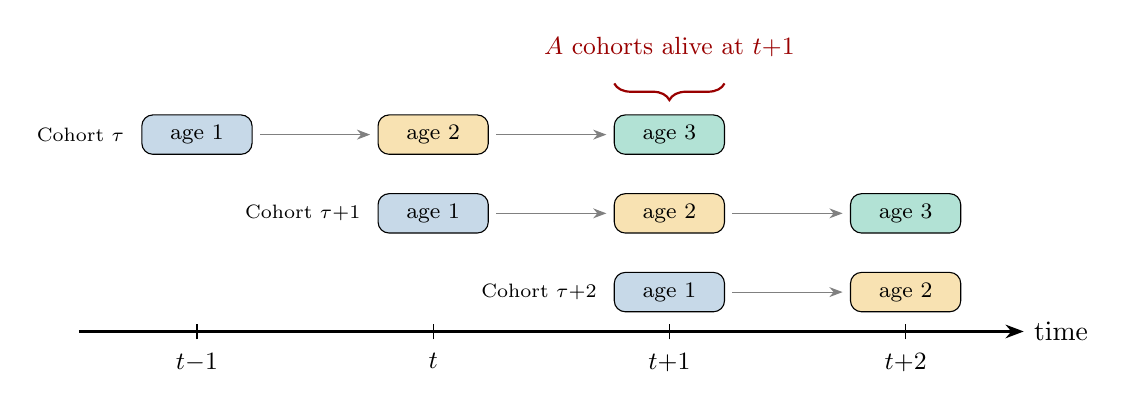
\begin{tikzpicture}[
    agent/.style={draw, rounded corners, minimum width=1.4cm, minimum height=0.5cm, font=\footnotesize},
    young/.style={agent, fill=softblue!30},
    mid/.style={agent, fill=softorange!30},
    old/.style={agent, fill=softgreen!30},
    >=Stealth
]
% Time axis
\draw[->, thick] (-0.5,0) -- (11.5,0) node[right] {time};
\foreach \t/\lab in {1/t{-}1, 4/t, 7/t{+}1, 10/t{+}2} {
    \draw (\t, -0.1) -- (\t, 0.1);
    \node[below] at (\t, -0.15) {\small $\lab$};
}

% Cohort 1 (born t-1)
\node[young] at (1, 2.5) {age 1};
\node[mid]   at (4, 2.5) {age 2};
\node[old]   at (7, 2.5) {age 3};
\draw[->, gray] (1.8, 2.5) -- (3.2, 2.5);
\draw[->, gray] (4.8, 2.5) -- (6.2, 2.5);
\node[left, font=\scriptsize] at (0.2, 2.5) {Cohort $\tau$};

% Cohort 2 (born t)
\node[young] at (4, 1.5) {age 1};
\node[mid]   at (7, 1.5) {age 2};
\node[old]   at (10, 1.5) {age 3};
\draw[->, gray] (4.8, 1.5) -- (6.2, 1.5);
\draw[->, gray] (7.8, 1.5) -- (9.2, 1.5);
\node[left, font=\scriptsize] at (3.2, 1.5) {Cohort $\tau{+}1$};

% Cohort 3 (born t+1)
\node[young] at (7, 0.5) {age 1};
\node[mid]   at (10, 0.5) {age 2};
\draw[->, gray] (7.8, 0.5) -- (9.2, 0.5);
\node[left, font=\scriptsize] at (6.2, 0.5) {Cohort $\tau{+}2$};

% Brace marking the t+1 column, placed above the diagram so it never
% crosses the inter-cohort transition arrows.
\draw[decorate, decoration={brace, amplitude=6pt, mirror}, thick, harvardcrimson]
    (6.3, 3.15) -- (7.7, 3.15)
    node[midway, above=6pt, font=\small, text=harvardcrimson]
    {$A$ cohorts alive at $t{+}1$};
\end{tikzpicture}

\vspace{0.3em}
At each period $t$ we have $A$ coexisting cohorts.  A newborn enters (age 1); the oldest dies (age $A$).\\
\emphc{Key observation:} the number of types is finite ($A$), so the cross-sectional state is finite-dimensional.
\end{frame}


\begin{frame}{The DEQN Recipe in One Line}
\small
\begin{block}{From model to neural network (to be applied twice in today's lecture)}
\begin{enumerate}\itemsep2pt
    \item Write down the \emphc{economic model}: preferences, technology, constraints, shocks.
    \item Define the \emphc{equilibrium}: choices + prices that satisfy optimization + market clearing.
    \item Write the \emphc{equilibrium conditions} as a system $G(x, f(x)) = 0$.
    \item Replace $f$ by a \emphc{neural network} $\N_\rho$ and form the \emphc{cost function} $\Loss(\rho) = \frac{1}{|D|}\sum_j \|G(x_j, \N_\rho(x_j))\|^2$.
    \item Sample training states $D$, minimize $\Loss(\rho)$ by SGD.
\end{enumerate}
\end{block}

\begin{alertblock}{The only thing that depends on the model}
The \emphc{equilibrium conditions $G$}.  Everything else -- the network, the SGD loop, the sampling method -- is generic.  \emphc{So to solve a new model, write down its $G$.}
\end{alertblock}

\vspace{0.2em}
{\footnotesize Today's deliverable: derive $G$ explicitly for both the analytic and the benchmark OLG models.}
\end{frame}


% =====================================================================
% Part II -- Analytic 6-agent model (Krueger & Kubler 2004)
% =====================================================================

\section{Part II: Analytic 6-agent OLG (Krueger \& K\"ubler, 2004)}

% --- II.1 Setup --------------------------------------------------------
\begin{frame}{II.1 Setup --- the Analytic Model}
\footnotesize
\begin{columns}[T]
\column{0.58\textwidth}
\begin{itemize}\itemsep1pt
    \item Time discrete: $t = 0, 1, 2, \ldots, \infty$.
    \item Agents live for $A = \emphc{6}$ periods.
    \item \emphc{One representative household per cohort}; a new one is born every period.
    \item \emphc{No uncertainty about lifetime}: all agents live exactly $A$ periods.
    \item Exogenous aggregate shock $z_t \in \{1,2,3,4\}$ drawn \emphc{i.i.d.}\ with transition $\pi_{ss'} = 0.25$.
    \item \emphc{Log utility} $u(c) = \ln c$ -- chosen because it gives a \emphc{closed-form} equilibrium (Krueger \& K\"ubler, 2004).
    \item \emphc{Labor:} only the youngest cohort works: $\ell^1 = 1,\ \ell^s = 0$ for $s \ge 2$.
\end{itemize}

\column{0.41\textwidth}
\begin{block}{Shocks: $z_t = (\eta_t, \delta_t)$}
{\scriptsize\renewcommand{\arraystretch}{0.95}
\begin{tabular}{cccc}
\toprule
$z$ & $\eta(z)$ & $\delta(z)$ & $\pi$\\
\midrule
1 & 0.95 & 0.5 & 0.25\\
2 & 1.05 & 0.5 & 0.25\\
3 & 0.95 & 0.9 & 0.25\\
4 & 1.05 & 0.9 & 0.25\\
\bottomrule
\end{tabular}}
\end{block}

\begin{block}{Calibration}
{\scriptsize $\alpha = 0.3,\;\beta = 0.7,\;\gamma = 1$ (log); $\underline{a}=0$.}
\end{block}
\end{columns}
\end{frame}


% --- II.2 Households I -------------------------------------------------
\begin{frame}{II.2 Households --- Preferences and the Savings Technology}
\small
Agents supply their labor \emphc{inelastically} for a market wage $w_t$.

\vspace{0.6em}
An agent \emphc{currently of age $s$} alive at $t$ maximises remaining time-separable discounted expected lifetime utility ($\beta < 1$):
\[
\E{\sum_{i=0}^{A-s} \beta^i \,\ln\!\bigl(c_{t+i}^{\,s+i}\bigr)} \qquad (1)
\]

\vspace{0.3em}
Households can save a unit of consumption to obtain a unit of capital good next period, denoted $a_t^s$.

\vspace{0.4em}
The savings become \emphc{capital in the next period}:
\[
a_t^{\,s} \;=\; k_{t+1}^{\,s+1}, \qquad \forall t,\ \forall s \in \{1, \ldots, A-1\}. \qquad (2)
\]
\end{frame}


% --- II.3 Households II ------------------------------------------------
\begin{frame}{II.3 Households --- Constraints, Budget, Boundary}
\small
Households \emphc{cannot die with debt}.  Borrowing is bounded:
\[
a_t^{\,s} \;\ge\; \underline{a}. \qquad (3)
\]
In the analytic model we set $\underline{a} = 0$: \emphc{no borrowing} for any cohort.

\vspace{0.4em}
At time $t$, households sell their capital to the firm at market price $r_t > 0$.  The per-period \emphc{budget constraint} of cohort $s$ reads
\[
c_t^{\,s} \;+\; a_t^{\,s} \;=\; r_t\, k_t^{\,s} \;+\; \ell^s\, w_t. \qquad (4)
\]

\vspace{0.4em}
\emphc{Boundary conditions.}  Newborns enter with no inheritance, and the oldest cohort dies without saving anything:
\[
k_t^{\,1} \;=\; 0, \qquad\qquad a_t^{\,A} \;=\; 0.
\]
\end{frame}


% --- II.4 Firms & Markets ----------------------------------------------
\begin{frame}{II.4 Firms and Markets}
\small
There is a single representative firm with \emphc{Cobb--Douglas} production.

\vspace{0.3em}
TFP $\eta$ and depreciation $\delta$ depend on the exogenous shock $z$ alone (see II.1 table).

\vspace{0.3em}
Each period, \emphc{after the shock has realized}, the firm buys capital and hires labor to maximize profits, taking prices as given.

\vspace{0.4em}
The stochastic production function is
\[
f(K, L, z) \;=\; \eta(z)\, K^\alpha\, L^{1-\alpha} \;+\; K\bigl(1-\delta(z)\bigr).
\]

\vspace{0.4em}
There are \emphc{competitive spot markets} for the consumption good, capital, and labor.

\vspace{0.5em}
{\footnotesize In the analytic model $L_t = \sum_{s=1}^A \ell^s = 1$ (only age-1 works), so the firm problem reduces to $\max_{K \ge 0} \eta(z) K^\alpha - (r_t - (1-\delta(z))) K$.}
\end{frame}


% --- II.5 Equilibrium definition ---------------------------------------
\begin{frame}{II.5 Competitive Equilibrium --- Definition}
\footnotesize
\begin{block}{Definition 1 (competitive equilibrium)}
\vspace{-2pt}
Given initial conditions $z_0,\,\{k_0^{\,s}\}_{s=1}^{A-1}$, a competitive equilibrium is a collection of choices for households $\bigl\{(c_t^{\,s},\,a_t^{\,s})_{s=1}^{A}\bigr\}_{t=0}^{\infty}$, for the representative firm $(K_t, L_t)_{t=0}^{\infty}$, and prices $(r_t, w_t)_{t=0}^{\infty}$, such that:
\begin{enumerate}\itemsep1pt
    \item Given $(r_t, w_t)_{t\ge 0}$, household choices maximize the lifetime utility (1) subject to the savings-to-capital identity (2), the borrowing limit (3), and the per-period budget (4):\\[1pt]
    \mbox{}\hspace{1em}{\scriptsize $a_t^{\,s} = k_{t+1}^{\,s+1};\;\; a_t^{\,s} \ge \underline{a};\;\; c_t^{\,s} + a_t^{\,s} = r_t k_t^{\,s} + \ell^s w_t.$}
    \item Given $(r_t, w_t)$, the firm maximises profits:\\[1pt]
    \mbox{}\hspace{1em}$(K_t, L_t) \in \arg\max_{K, L \ge 0} f(K, L, z_t) - r_t K - w_t L$.
    \item \emphc{All markets clear:} for all $t$,\;\, $L_t = \sum_{s=1}^A \ell^s, \;\; K_t = \sum_{s=1}^A k_t^{\,s}.$
\end{enumerate}
\vspace{-2pt}
\end{block}
\end{frame}


% --- II.6 Equilibrium conditions ---------------------------------------
\begin{frame}{II.6 Equilibrium Conditions}
\small
\textbf{Firm FOCs} (closed form from Cobb--Douglas):
\[
w_t \;=\; (1-\alpha)\,\eta(z_t)\, K_t^{\alpha}\, L_t^{-\alpha}, \qquad
r_t \;=\; \alpha\,\eta(z_t)\, K_t^{\alpha-1}\, L_t^{1-\alpha} \;+\; \bigl(1-\delta(z_t)\bigr).
\]

\vspace{0.3em}
\textbf{Household optimality} for any cohort of age $s \in \{1, \ldots, A-1\}$ (FOC in $c_t^{\,s}$ gives $\nu_t^s = u'(c_t^{\,s})$; FOC in $a_t^{\,s}$ gives the standard \emphc{interior} Euler equation):
\[
\boxed{\;\underbrace{u'\!\bigl(c_t^{\,s}\bigr)}_{=\,1/c_t^{\,s}\text{ since }u=\ln} \;=\; \beta\;\E{u'\!\bigl(c_{t+1}^{\,s+1}\bigr)\,r_{t+1}}\;}
\]

\vspace{0.3em}
\textbf{Terminal cohort.}  Age $A$: consume everything, save nothing.

\vspace{0.3em}
{\scriptsize \emphc{Why no KKT multiplier?}  In this calibration ($\gamma=1$, $\beta=0.7$, only the youngest cohort works) the borrowing constraint $a_t^{\,s}\ge 0$ never binds in equilibrium, so $\lambda_t^{\,s}\equiv 0$ and drops out of the Euler equation, the FREE signature, and the loss.  Part III re-introduces multipliers for the binding constraints of the 56-cohort benchmark.}
\end{frame}


% --- II.7 Cost function ------------------------------------------------
\begin{frame}{II.7 The DEQN Cost Function}
\small
\begin{block}{Explicit cost function}
\[
\boxed{\;\Loss_{D_{\text{train}}}(\rho) \;:=\; \frac{1}{|D_{\text{train}}|}\;\frac{1}{A-1}\,
\sum_{x_j \in D_{\text{train}}}\;\sum_{i=1}^{A-1} \bigl(e_{\text{REE}}^{\,i}(x_j)\bigr)^2\;}
\]
\end{block}

\vspace{0.3em}
\textbf{Relative Euler-equation residual} (cohort $i$):
\[
e_{\text{REE}}^{\,i}(x_j) \;:=\;
\frac{\Bigl(u'\Bigr)^{-1}\!\!\left(\beta\,\E{r\bigl(\hat x_{j,+}\bigr)\,u'\bigl(\hat c^{\,i+1}(\hat x_{j,+})\bigr)}\right)}{\hat c^{\,i}(x_j)} \;-\; 1.
\]

\vspace{0.2em}
\textbf{Sampling next state.}  $\hat x_{j,+} = \bigl(z_+,\; 0,\; \hat a^{\,[1:A-1]}(x_j)\bigr)$ with $z_+$ drawn from $\pi$ (newborn enters with $k^1 = 0$).

\vspace{0.2em}
{\scriptsize \emphc{Feasibility.}  $a^s\ge 0$ is enforced by the softplus output of II.9; small soft penalties on negative $c$ and $K$ are added in the notebook for numerical robustness only -- they vanish at convergence.}
\end{frame}


% --- II.8 Functional Rational Expectations Equilibrium ----------------
\begin{frame}{II.8 Functional Rational Expectations Equilibrium (FREE)}
\footnotesize
\begin{exampleblock}{FREE: one function that solves the equilibrium conditions at every state}
\vspace{-2pt}
\textbf{Signature:}\;
$
f:\;\{1,2,3,4\}\times \R^{A} \;\longrightarrow\; \R^{\,A-1},
$\quad input $=$ state $(z_t, \bm{k}_t)$, output $=$ savings policies.

\vspace{2pt}
\textbf{Output decomposition} ($A-1$ scalars):
\[
f\!\left(\!\begin{bmatrix} z_t \\ \bm{k}_t \end{bmatrix}\!\right)
\;=\;
\bigl[\,\underbrace{a_t^{\,1},\,a_t^{\,2},\,\ldots,\,a_t^{\,A-1}}_{\text{capital-investment policies}}\,\bigr]^{\!\top}.
\]
\end{exampleblock}

\textbf{Such that, for all cohorts $s = 1, \ldots, A-1$, the (interior) Euler equation holds:}
\[
\beta\,\E{\frac{r_{t+1}\,u'(c_{t+1}^{\,s+1})}{u'(c_t^{\,s})}} - 1 \;=\; 0 \qquad (\text{Euler residual}).
\]
Stack these $A-1$ residuals as $G\bigl([z_t, \bm{k}_t],\, f([z_t, \bm{k}_t])\bigr) = \bm{0}$.

{\scriptsize $A=6 \Rightarrow 5$ outputs.  Notebook uses an extended state of dim $8+4A=32$ (pre-computed aggregates + per-agent income blocks) for ease of learning -- pure feature engineering.}
\end{frame}


% --- II.9 Architecture --------------------------------------------------
\begin{frame}{II.9 Deep Equilibrium Net --- Architecture (Analytic)}
\small
\begin{columns}[T,totalwidth=0.96\textwidth]
\column{0.46\textwidth}
\[
\N_\rho:\;\{1,2,3,4\}\times\R^A \to \R^{A-1}
\]
\[
\N_\rho\!\left(\!\begin{bmatrix} z_t \\ \bm{k}_t\end{bmatrix}\!\right) \;=\;
\left[
\begin{array}{l}
a_t^{\,1}\\ a_t^{\,2}\\ \vdots\\ a_t^{\,A-1}
\end{array}
\right]
\]
such that
\[
G\!\left(\!\begin{bmatrix} z_t \\ \bm{k}_t\end{bmatrix},\; \N_\rho\!\left(\!\begin{bmatrix} z_t \\ \bm{k}_t\end{bmatrix}\!\right)\right) \;\approx\; \bm{0}.
\]
{\footnotesize \emphc{Softplus} output layer $\Rightarrow$ $a_t^{\,s} \ge 0$ \emphc{by construction}, so the borrowing constraint is satisfied at every iteration without an explicit multiplier.}

\column{0.48\textwidth}
\centering
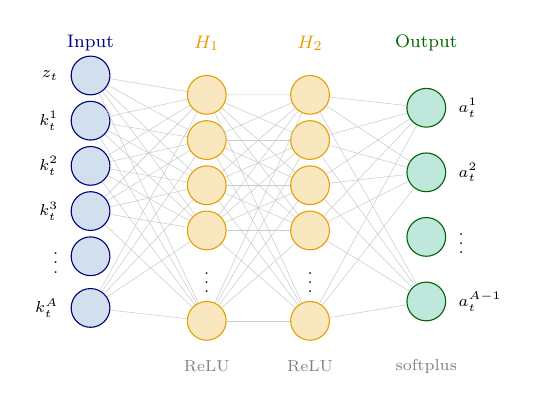
\begin{tikzpicture}[scale=0.82, every node/.style={transform shape},
    inn/.style={circle, draw=uzhblue, fill=softblue!25, minimum size=6mm, inner sep=0pt, font=\scriptsize},
    hd/.style={circle, draw=softorange, fill=softorange!25, minimum size=6mm, inner sep=0pt, font=\scriptsize},
    outt/.style={circle, draw=darkgreen, fill=softgreen!25, minimum size=6mm, inner sep=0pt, font=\scriptsize},
    dots/.style={font=\scriptsize},
    >=Stealth
]
\node[font=\footnotesize, uzhblue]     at (0, 3.4) {Input};
\node[font=\footnotesize, softorange]  at (1.8, 3.4) {$H_1$};
\node[font=\footnotesize, softorange]  at (3.4, 3.4) {$H_2$};
\node[font=\footnotesize, darkgreen]   at (5.2, 3.4) {Output};

\foreach \i/\y/\lab in {a/2.9/$z_t$, b/2.2/$k^1_t$, c/1.5/$k^2_t$, d/0.8/$k^3_t$, e/0.1/$\vdots$, f/-0.7/$k^A_t$} {
    \node[inn] (In\i) at (0, \y) {};
    \node[left=2pt of In\i, font=\scriptsize] {\lab};
}

\foreach \i/\y in {a/2.6, b/1.9, c/1.2, d/0.5, e/-0.9} {
    \node[hd] (HOne\i) at (1.8, \y) {};
    \node[hd] (HTwo\i) at (3.4, \y) {};
}
\node[dots] at (1.8, -0.2) {$\vdots$};
\node[dots] at (3.4, -0.2) {$\vdots$};

\foreach \i/\y/\lab in {a/2.4/$a_t^1$, b/1.4/$a_t^2$, c/0.4/$\vdots$, d/-0.6/$a_t^{A-1}$} {
    \node[outt] (Out\i) at (5.2, \y) {};
    \node[right=2pt of Out\i, font=\scriptsize] {\lab};
}

% connections input -> H1
\foreach \a in {a, b, c, d, f}
    \foreach \b in {a, b, c, d, e}
        \draw[gray!40, very thin] (In\a) -- (HOne\b);
% H1 -> H2
\foreach \a in {a, b, c, d, e}
    \foreach \b in {a, b, c, d, e}
        \draw[gray!40, very thin] (HOne\a) -- (HTwo\b);
% H2 -> output
\foreach \a in {a, b, c, d, e}
    \foreach \b in {a, b, d}
        \draw[gray!40, very thin] (HTwo\a) -- (Out\b);

\node[font=\scriptsize, gray] at (1.8, -1.6) {ReLU};
\node[font=\scriptsize, gray] at (3.4, -1.6) {ReLU};
\node[font=\scriptsize, gray] at (5.2, -1.6) {softplus};
\end{tikzpicture}

{\footnotesize 2 hidden layers $\times$ (100, 50) units; single forward pass.}
\end{columns}
\end{frame}


% --- Hand-over to the analytic-model notebook -------------------------
\begin{frame}{Companion Notebook Hand-over}
\scriptsize
\emphc{Open notebook 07.}  It implements the model, equilibrium conditions, loss, FREE map, architecture, training, and validation covered in Part II.
\vspace{-2pt}
\begin{block}{Cell-to-slide map}
\vspace{-4pt}
\begin{center}\renewcommand{\arraystretch}{0.85}
{\scriptsize
\begin{tabular}{ll}
\toprule
\textbf{Deck slide} & \textbf{Notebook section} \\
\midrule
II.1--II.6 Model and equilibrium        & \S 1--5 \;calibration, prices, residuals \\
II.7--II.9 Loss, FREE, architecture     & \S 6--7 \;\texttt{compute\_cost()}, \texttt{build\_network()} \\
II.10--II.13 Training/validation        & \S 8--10 \;cloud method + closed-form checks \\
\bottomrule
\end{tabular}}
\end{center}
\vspace{-4pt}
\end{block}
\end{frame}


% --- II.10 Sampling + training loop -----------------------------------
\begin{frame}{II.10 Sampling and the Training Loop}
\small
\begin{block}{Cloud method (Azinovic, Gaegauf \& Scheidegger, 2022)}
\vspace{-2pt}
\begin{enumerate}\itemsep2pt
    \item \emphc{Initialisation.}  Sample a cloud of initial states $D_0 = \{x_j^{\,0}\}_{j=1}^{N}$; initialise $\rho^0$.
    \item \emphc{Episode $k$.}
    \begin{enumerate}
        \item[(a)] \textbf{Simulate.}  Draw fresh shocks $\{z_{+,j}\}$ from $\pi$; roll the cloud forward one period using the \emphc{current} policy $\N_{\rho^k}$:
        $x_j^{\,k+1} = \bigl(z_{+,j},\,0,\,\N_{\rho^k}^{[1:A-1]}(x_j^{\,k})\bigr)$.
        \item[(b)] \textbf{Mini-batch SGD.}  Take $\texttt{steps}$ Adam steps on $\Loss_{D_k}(\rho)$ using mini-batches from $D_k$.
    \end{enumerate}
    \item \emphc{Stop} when $\log_{10} \Loss$ falls below the target.
\end{enumerate}
\end{block}

\vspace{0.2em}
\textbf{Definitions.}  \emphc{Episode} = one simulate-then-train pass.  \emphc{Epoch} = one pass through the full cloud.

\vspace{0.3em}
{\footnotesize Sampling from the ergodic set of the current policy makes the cost function focus on states the economy actually visits.}
\end{frame}


% --- II.11 Training results -------------------------------------------
\begin{frame}{II.11 Training Results --- Analytic Model}
\small
\centering
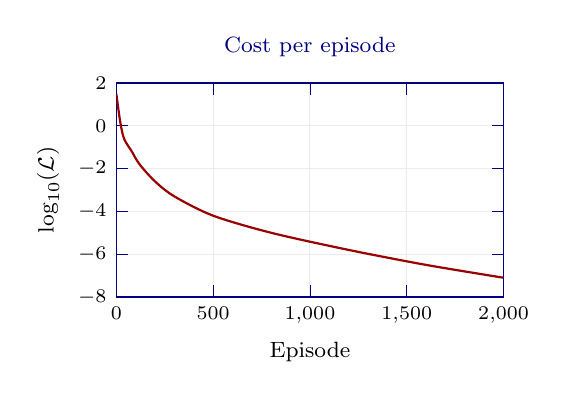
\begin{tikzpicture}
\begin{axis}[
    width=6.5cm, height=4.3cm,
    xlabel={Episode}, ylabel={$\log_{10}(\Loss)$},
    xmin=0, xmax=2000, ymin=-8, ymax=2,
    grid=major, grid style={gray!15},
    axis line style={uzhblue}, tick style={uzhblue},
    label style={font=\footnotesize}, ticklabel style={font=\scriptsize},
    title style={font=\footnotesize, uzhblue},
    title={Cost per episode}
]
\addplot[harvardcrimson, thick, smooth] coordinates {
    (0,1.5) (20,0.2) (40,-0.6) (80,-1.2) (120,-1.8)
    (200,-2.6) (300,-3.3) (500,-4.2) (800,-5.0) (1200,-5.8)
    (1600,-6.5) (2000,-7.1)
};
\end{axis}
\end{tikzpicture}
\hfill
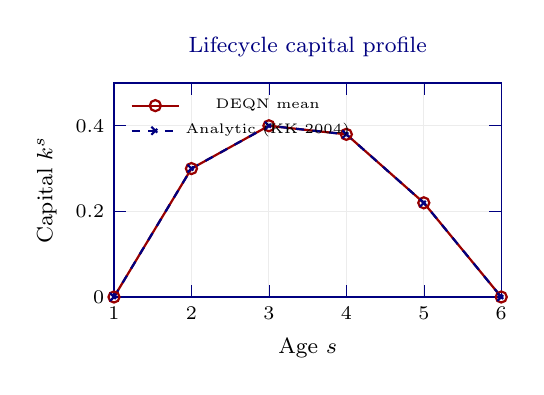
\begin{tikzpicture}
\begin{axis}[
    width=6.5cm, height=4.3cm,
    xlabel={Age $s$}, ylabel={Capital $k^s$},
    xmin=1, xmax=6, ymin=0, ymax=0.5,
    xtick={1,2,3,4,5,6},
    grid=major, grid style={gray!15},
    axis line style={uzhblue}, tick style={uzhblue},
    label style={font=\footnotesize}, ticklabel style={font=\scriptsize},
    title style={font=\footnotesize, uzhblue},
    title={Lifecycle capital profile},
    legend style={font=\tiny, draw=none, fill=none, at={(0.02,0.98)}, anchor=north west}
]
\addplot[harvardcrimson, thick, mark=o, mark options={solid}] coordinates {
    (1,0.00) (2,0.30) (3,0.40) (4,0.38) (5,0.22) (6,0.00)
};
\addlegendentry{DEQN mean}
\addplot[uzhblue, thick, dashed, mark=x] coordinates {
    (1,0.00) (2,0.30) (3,0.40) (4,0.38) (5,0.22) (6,0.00)
};
\addlegendentry{Analytic (KK 2004)}
\end{axis}
\end{tikzpicture}

\vspace{0.15em}
\begin{block}{Reading the plots}
\emphc{Left:} cost falls in $\log_{10}$ as the network learns the Krueger--K\"ubler policy; classroom is diagnostic, production reaches tight residuals.\\
\emphc{Right:} trained DEQN savings policy overlays the closed-form Krueger--K\"ubler solution across cohorts.
\end{block}
\end{frame}


% --- II.12 Finger exercise --------------------------------------------
\begin{frame}{\emphc{Finger Exercise:} Closed-Form Savings Rates}
\small
\textbf{Setup.}  With $u = \ln$, cohort $h$'s Euler equation reads $1/c_t^h = \beta\,\mathbb{E}_t[r_{t+1}/c_{t+1}^{h+1}]$ and the budget constraint is $c_t^h + a_t^h = \text{inc}_t^h$ where $\text{inc}_t^h = r_t k_t^h + \ell^h w_t$.  (The household-level setup slides II.2--II.6 used the index symbol $s$; from this slide onward we follow the script convention and use $h$ instead.)

\vspace{0.4em}
\textbf{Claim (Krueger \& K\"ubler, 2004).}  With log utility and 100\% consumption at age $A$, the savings rate $\beta_h := a_t^h/\text{inc}_t^h$ of cohort $h$ depends only on age:
\[
\beta_h \;=\; \beta\,\frac{1 - \beta^{A-h}}{1 - \beta^{A-h+1}}, \qquad h = 1, \ldots, A-1.
\]

\vspace{0.4em}
\textbf{Task (3 minutes).}  Compute $\beta_1, \beta_2, \ldots, \beta_5$ with $\beta = 0.7$.  Interpret:
\begin{itemize}
\item What happens as cohorts approach retirement?
\item Why are younger cohorts saving more as a \emphc{rate}?
\end{itemize}
\end{frame}


\begin{frame}{\emphc{Solution:} Closed-Form Savings Rates}
\footnotesize
\[
\beta_h \;=\; 0.7 \cdot \frac{1 - 0.7^{\,6-h}}{1 - 0.7^{\,7-h}}
\]

\vspace{-0.1em}
\begin{center}\renewcommand{\arraystretch}{0.95}
\begin{tabular}{ccc}
\toprule
Cohort $h$ & Periods remaining ($A-h$) & Savings rate $\beta_h$\\
\midrule
1 & 5 & $0.7\cdot(1-0.7^5)/(1-0.7^6) \approx 0.660$ \\
2 & 4 & $0.7\cdot(1-0.7^4)/(1-0.7^5) \approx 0.639$ \\
3 & 3 & $0.7\cdot(1-0.7^3)/(1-0.7^4) \approx 0.605$ \\
4 & 2 & $0.7\cdot(1-0.7^2)/(1-0.7^3) \approx 0.543$ \\
5 & 1 & $0.7\cdot(1-0.7)/(1-0.7^2) \approx 0.412$ \\
6 & 0 & $0$ (consumes everything)\\
\bottomrule
\end{tabular}\end{center}

\vspace{-0.1em}
\begin{block}{Interpretation}
\vspace{-3pt}\begin{itemize}\itemsep0pt
    \item Savings rate \emphc{monotonically declines} with age: as the horizon shrinks, saving less is optimal.
    \item Youngest cohort saves \emphc{$\sim 66\%$} of its income -- longest horizon to enjoy the returns.
    \item At $A$: terminal boundary $a^A = 0$ -- consume everything.
\end{itemize}
\end{block}
\end{frame}


% --- II.13 Validation --------------------------------------------------
\begin{frame}{II.13 DEQN vs.\ Analytical Solution}
\footnotesize
\centering
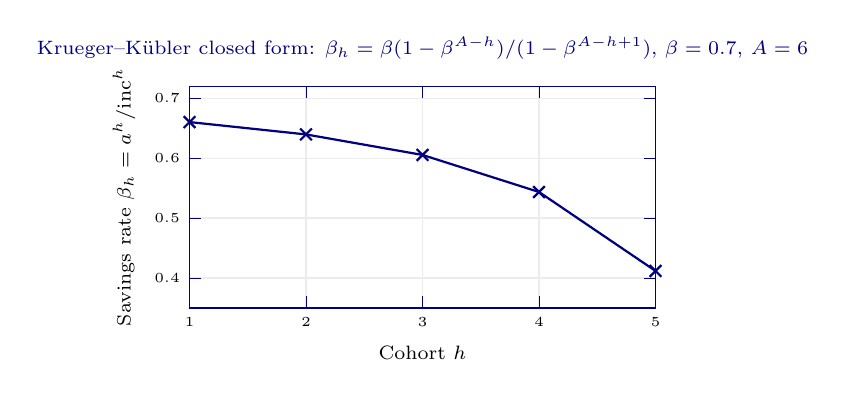
\begin{tikzpicture}
\begin{axis}[
    width=7.5cm, height=4.4cm,
    xlabel={Cohort $h$}, ylabel={Savings rate $\beta_h = a^h / \text{inc}^h$},
    xmin=1, xmax=5, ymin=0.35, ymax=0.72,
    xtick={1,2,3,4,5},
    grid=major, grid style={gray!15},
    axis line style={uzhblue}, tick style={uzhblue},
    label style={font=\scriptsize}, ticklabel style={font=\tiny},
    title style={font=\scriptsize, uzhblue},
    title={Krueger--K\"ubler closed form: $\beta_h = \beta(1-\beta^{A-h})/(1-\beta^{A-h+1})$, $\beta=0.7,\,A=6$}
]
\addplot[uzhblue, thick, mark=x, mark size=3pt] coordinates {
    (1,0.6600) (2,0.6394) (3,0.6052) (4,0.5434) (5,0.4118)
};
\end{axis}
\end{tikzpicture}

\vspace{0.2em}
\begin{block}{Validation strategy}
\vspace{-2pt}
The plotted points are the \emphc{exact closed form} from the finger-exercise solution slide.  The DEQN should reproduce this curve cohort-by-cohort.

\vspace{2pt}
The actual training run, DEQN-vs-analytic comparison, and Euler-error histogram are produced by notebook 07 (\S 10).  Production target in AGS (2022): mean relative Euler error $\lesssim 10^{-3}$.
\end{block}
\end{frame}


\begin{frame}{II Take-away and Hands-on}
\footnotesize
\begin{block}{What we just did}
\begin{enumerate}\itemsep1pt
    \item OLG model with 6 cohorts, log utility, 4 i.i.d.\ shocks (II.1--II.4).
    \item Equilibrium definition + conditions (II.5--II.6).
    \item Conditions $\to$ \emphc{cost function} (II.7).
    \item Equilibrium map $f$ $\to$ neural network $\N_\rho$ (II.8--II.9).
    \item Trained by sampling + SGD (II.10--II.11), \emphc{validated} against the closed form (II.13).
\end{enumerate}
\end{block}

\begin{block}{Hands-on}
Open notebook 07.  Default \texttt{MODE = "classroom"} ($\sim 5$ min, 1\,000 ep); \texttt{"smoke"} is a 30-s sanity check; \texttt{"production"} chases AGS Table~3 accuracy.
\end{block}
\end{frame}



\end{document}
